\documentclass[12pt]{article}

\usepackage[utf8]{inputenc}
\usepackage[T1]{fontenc}
\usepackage[slovak]{babel}
\usepackage{hyperref}
\usepackage{graphicx}
\usepackage{tabularx}
\usepackage{amsthm}
\usepackage{amsfonts}
\usepackage{url}
\usepackage[a4paper,top=2.5cm,bottom=2.5cm,left=3.5cm,right=2cm]{geometry}
\linespread{1.25}

\DeclareUnicodeCharacter{0161}{\v{s}} % š
\DeclareUnicodeCharacter{010D}{\v{c}} % č
\DeclareUnicodeCharacter{0165}{\v{t}} % ť
\DeclareUnicodeCharacter{010F}{\v{d}} % ď
\DeclareUnicodeCharacter{013E}{\v{l}} % ľ
\DeclareUnicodeCharacter{00E1}{\'{a}} % á
\DeclareUnicodeCharacter{00E9}{\'{e}} % é
\DeclareUnicodeCharacter{00FD}{\'{y}} % ý
\DeclareUnicodeCharacter{00F3}{\'{o}} % ó

\DeclareUnicodeCharacter{0160}{\v{S}} % Š
\DeclareUnicodeCharacter{010C}{\v{C}} % Č
\DeclareUnicodeCharacter{0164}{\v{T}} % Ť
\DeclareUnicodeCharacter{010E}{\v{D}} % Ď
\DeclareUnicodeCharacter{013D}{\v{L}} % Ľ
\DeclareUnicodeCharacter{00C1}{\'{A}} % Á
\DeclareUnicodeCharacter{00C9}{\'{E}} % É
\DeclareUnicodeCharacter{00DD}{\'{Y}} % Ý
\DeclareUnicodeCharacter{00D3}{\'{O}} % Ó

\begin{document}
	\title{\textbf{Teória čísel pre ZŠ}}
	
	
	\date{\today}
	\author{}
	%\institute{}
	\maketitle
	\begin{center}
		
\includegraphics[width=6cm]{assets/educat.jpg}
	\end{center}
	\tableofcontents
	\newpage
	
	\section{Čísla a ich základné typy}
	\subsection{Číslo a cifra}
	Do obrázku a textu pod ním doplň slová \textbf{cifra} a \textbf{číslo} podľa významu.\\
	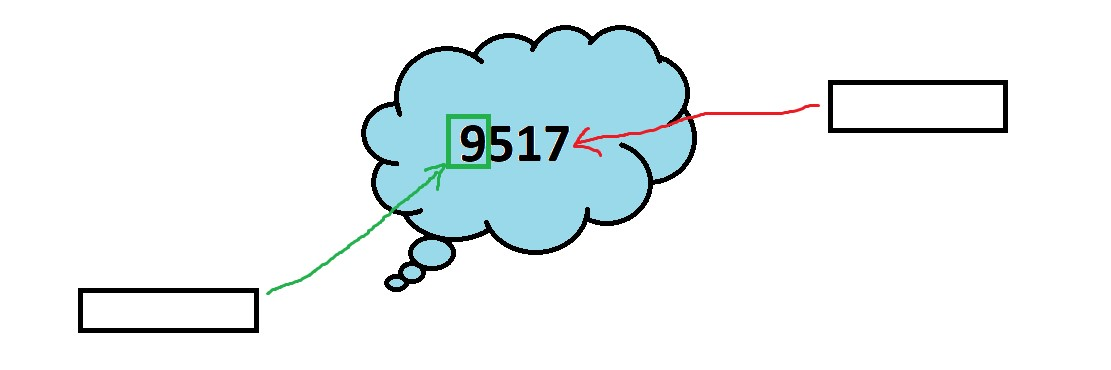
\includegraphics[width=14cm]{assets/cifra_vs_cislo} 
	\newline
	\textbf{Definície:}
	\begin{itemize}
		\item $\underline{\hspace{2cm}}$ je matematický objekt, ktorý sa používa na počítanie, meranie a označovanie.
		\item $\underline{\hspace{2cm}}$ je grafický objekt, ktorý sa používa na znázorňovanie čísel a môže nadobúdať hodnoty $\underline{\hspace{3cm}}$.
	\end{itemize}
	
	\subsection{Základné matematické operácie a ich vlastnosti}
	Z tabuľky doplň slová do textu pod ňou. Do zátvoriek napíš názov danej operácie.\\
	\begin{table}[!hbt]
		\centering
		\begin{tabular}{|cccc|}
			\hline
			asociatívnosť& násobenie& sčitovanie& komutatívnosť \\
			
			distributívnosť& delenie& odčitovanie& neutrálny prvok\\
			
			sčítanec& činiteľ& delenec& deliteľ\\
			
			súčet& podiel& súčin& rozdiel\\
			
			menšenec& menšiteľ& opačné číslo& \\
			
			\hline
		\end{tabular}
		
	\end{table}
	\\
	$\underline{\hspace{4cm}} + \underline{\hspace{4cm}} = \underline{\hspace{4cm}} (\underline{\hspace{2cm}})$\\
	
	$\underline{\hspace{4cm}} - \underline{\hspace{4cm}} = \underline{\hspace{4cm}}  (\underline{\hspace{2cm}})$\\
	
	$\underline{\hspace{4cm}} $.$ \underline{\hspace{4cm}} = \underline{\hspace{4cm}}  (\underline{\hspace{2cm}})$\\
	
	$\underline{\hspace{4cm}} \div \underline{\hspace{4cm}}
	= \underline{\hspace{4cm}} (\underline{\hspace{2cm}})$\\
	\newline
	\textbf{Vlastnosti základných matematických operácií:}\\
	\begin{itemize}
		\item $a+b = b+a$, $a.b = b.a$ ($\underline{\hspace{2cm}}$)
		\item $a.1 = 1.a = a, a+0 = 0+a = 0$ ($\underline{\hspace{3cm}}$)
		\item $a-b = 0$, potom $b$ sa nazýva $\underline{\hspace{3cm}}$.
		\item $a.(x+y) = a.x + b.y$ ($\underline{\hspace{3cm}}$)
		\item $(a+b)+c = a+(b+c), (a.b).c = a.(b.c)$ ($\underline{\hspace{3cm}}$)
	\end{itemize}
	
	\subsection{Základné typy čísel}
	Do textu nižšie doplň správne slová z nasledujúcej tabuľky:
	\newline
	\begin{table}[!hbt]
		\centering
		\begin{tabular}{|cccc|}
			
			\hline
			prirodzené čísla &celé čísla &$\mathbb{N}$ &$\mathbb{Z}$ \\
			%\hline
			opačné &$\mathbb{N}_0$ &1, 2, 3 \dots &\dots, -2, -1, 0, 1, 2, 3, \dots\\
			
			\hline
			
		\end{tabular}
	\end{table}
	\begin{itemize}
		\item $\underline{\hspace{4cm}}$ sú čísla, ktoré vyjadrujú nenulový počet prvkov a na ich značenie používame znak $\underline{\hspace{2cm}}$. Patria sem napríklad čísla $\underline{\hspace{3cm}}$. Ak by sme ale chceli dať najavo, že počítame aj s nulou, použijeme značenie $\underline{\hspace{2cm}}$.
		\item naopak $\underline{\hspace{4cm}}$ sú také čísla, ktoré už nulu obsahujú. Vyjadrujú totiž zmenu (rast alebo pokles)  počtu prvkov. Obsahujú teda aj prirodzené čísla, nulu aj čísla k nim $\underline{\hspace{2cm}}$. Patria sem napríklad čísla $\underline{\hspace{4cm}}$ a požívame pre ne značenie $\underline{\hspace{2cm}}$.
	\end{itemize}
	
	\subsection{Zápisy prirodzených čísel}
	K nasledujúcim zápisom dopíš, aký majú názov.
	
	\begin{itemize}
		\item 543 - $\underline{\hspace{3cm}}$.
		\item $5.100 + 4.10 + 3.1$ -$\underline{\hspace{3cm}}$.
		\item $5.100~ + ~43$ - $\underline{\hspace{4cm}}$. V tomto prípade sa číslo $5.100$ nazýva $\underline{\hspace{2cm}}$ a číslo 43 $\underline{\hspace{4cm}}$.
		
	\end{itemize}
	
	\subsection{Cvičenie.} V nasledujúcej tabuľke máš v každom riadku daný práve 1 typ zápisu čísla, tvojou úlohou je dopísať zápisy vo zvyšných stĺpcoch (v treťom stĺpci číslo v zátvorke vyjadruje deliteľa, ktorého máš použiť).\newline
	
	\begin{table}[!hbt]
		
		\begin{tabular}{|l|l|l|}
			\hline
			Ciferný zápis& Rozvinutý zápis& Zápis pomocou zvyšku\\
			\hline
			&$3.1000 + 0.100 + 4.10 + 9.1$&(7) \\
			\hline
			221& &(10)\\
			\hline
			& & $7.8 + 4$\\
			\hline
			31& &(5)\\
			\hline
			76& &(12)\\
			\hline
			&$6.100 + 2.10 + 7.1$&(21)\\
			\hline
			& &$7.24 + 21$\\
			\hline
			214& &(15)\\
			\hline
			571& &(20)\\
			\hline
			&$3.100 + 4.10 + 7.1$ &(6)\\
			\hline
			&$7.1000 + 9.100 + 7.10 + 1.1$&(8)\\
			\hline
		\end{tabular}
	\end{table}
	
	\newpage
	\section{Deliteňosť celých a prirodzených čísel}
	
	\subsection{Definícia deliteľnosti}
	Ak si zoberieme 2 celé čísla a, b, tak povieme, že číslo a je $\underline{\hspace{2cm}}$ číslom b, ak nám po $\underline{\hspace{4cm}}$ výjde zvyšok 0. Hovoríme tiež, že b je $\underline{\hspace{2cm}}$ čísla a. Matematické značnie je potom, $a|b$ (a delí b). Inými slovami sa dá povedať, že a delí b, ak je b násobkom a-čka.\newline
	Treba si dať ale pozor, číslo a nesmie byť rovné $\underline{\hspace{2cm}}$.
	
	\subsection{Znaky deliteľnosti pre čísla 2, 3, 4, 5, 6, 8, 9, 10.}
	Pomocou učebnice alebo internetu doplň kritériá deliteľnosti pre spomänuté prirodzené čísla.\\
	
	\begin{enumerate}
		\item pridrodzené číslo je deliteľné 2, ak $\underline{\hspace{6cm}}$.
		\item pridrodzené číslo je deliteľné 3, ak $\underline{\hspace{6cm}}$.
		\item pridrodzené číslo je deliteľné 4, ak $\underline{\hspace{6cm}}$.
		\item pridrodzené číslo je deliteľné 5, ak $\underline{\hspace{6cm}}$.
		\item pridrodzené číslo je deliteľné 6, ak $\underline{\hspace{6cm}}$.
		\item pridrodzené číslo je deliteľné 8, ak $\underline{\hspace{6cm}}$.
		\item pridrodzené číslo je deliteľné 9, ak $\underline{\hspace{6cm}}$.
		\item pridrodzené číslo je deliteľné 10, ak $\underline{\hspace{6cm}}$.
	\end{enumerate}
	
	\subsection{Zisťovanie všetkých deliteľov}
	Predstav si, že nám niekto predostrie nejaké prirodzené číslo a chce od nás, aby sme mu povedali, koľko deliteľov dané číslo má, prípadne ešte aj, ktoré sú to čísla. Aký postup by sme na to mali zvoliť\newline
	
	\textbf{Postup:} $\underline{\hspace{10cm}}$
	\newline
	\subsection{Cvčenia}
	\url{https://gymmoldava.sk/ICV/CELYWEB/1/delitelnost/delitelnostkviz.htm}\\
	\url{https://gymmoldava.sk/ICV/CELYWEB/1/delitelnost/znakydelitelnosti.htm}\\
	\url{https://gymmoldava.sk/ICV/CELYWEB/1/delitelnost/znakydelitelnosti2.htm}
	
	\subsection{Prvočísla a prvočíselné rozklady}
	Z možností v texte vyber tie správne.
	\newline
	
	\qquad \textbf{Prvočíslo{/}zložené číslo} je také prirodzené číslo, ktoré má práve 2 delitele. Naopak, prirodzené číslo, ktoré má \textbf{aspoň{/}najviac} 3 delitele sa nazýva \textbf{prvočíslo{/}zložené číslo}. Z toho dôvodu číslo 1 nie je ani prvočíslo, ani zložené číslo, keďže má len 1 deliteľa.
	
	\subsection{Eratostenovo sito}
	
	\qquad 	Na hľadanie všetkých prvočísel existuje postup, ktorý vymyslel už ujo Eratostenes z Kyrény v antickom Grécku. Funguje tak, že si najprv vytvoríme štvorcovú tabuľku $n \times n$. Postup pozostáva z 5 krokov: 
	
	\begin{enumerate}
		\item Jednotku vyškrtni, ona nie je prvočíslom.
		\item Dvojku zafarbi, ona je prvočíslom.
		\item Vyškrtni všetky jej násobky (4, 6, 8, \dots)
		\item Zafarbi najmenšie nezvyškrtnuté číslo a opakuj s ním kroky 2 a 3.
		\item Toto opakuj, kým nemáš hotovú celú tabuľku.
	\end{enumerate}
	
	Teraz si tento postup vyskúšaj na štvorci $10 \times 10$, teda máš nájsť prvočísla od 1 po 100.
	\newline
	\begin{center}
		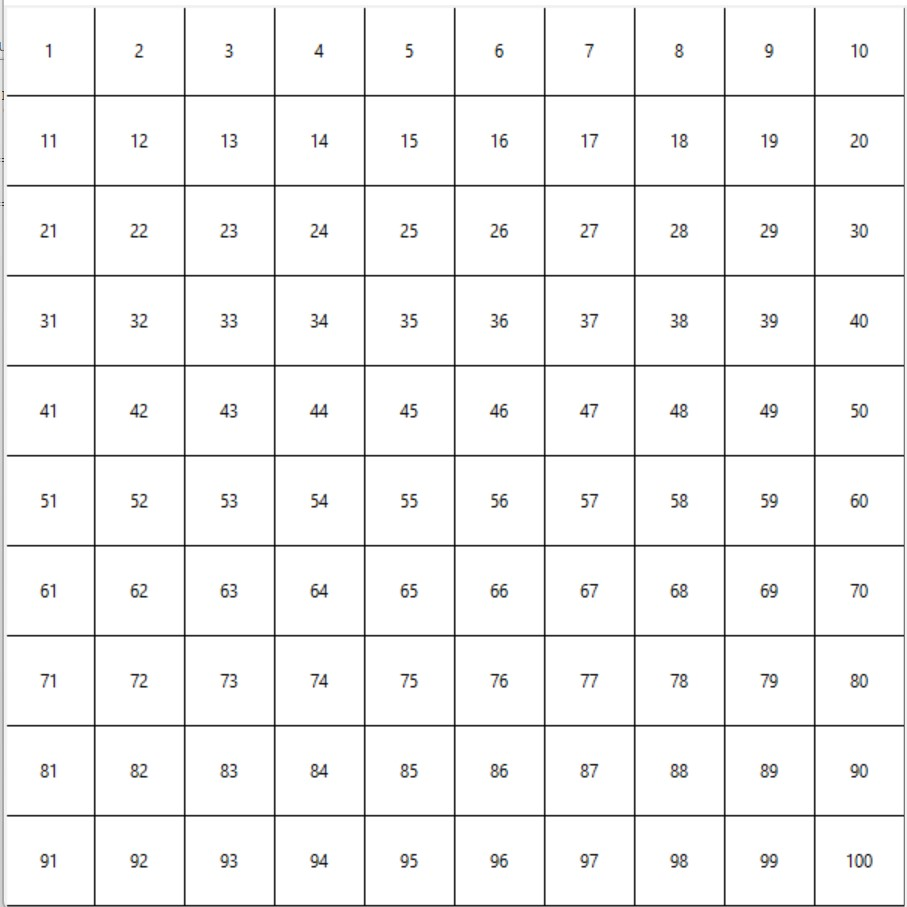
\includegraphics[width=10cm]{assets/prazdne_sito.jpg}
	\end{center}
	
	Po vyfarbení by mala tabuľka vyzerať takto (zelené sú prvočísla):
	\begin{center}
		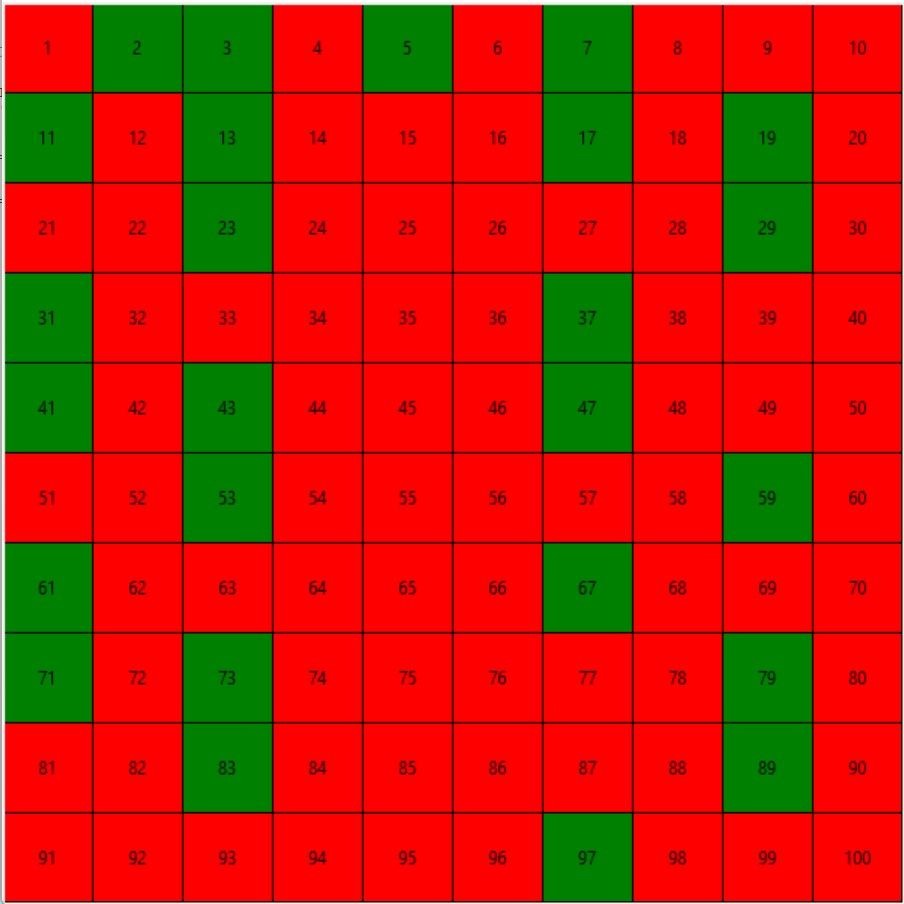
\includegraphics[width=10cm]{assets/vyfarbene_sito.jpg}
	\end{center}
	
	\subsection{Prvočíselný rozklad prirodzeného čísla}
	
	Do nasledujúceho textu doplň tieto slová: \textbf{prvočísel, prvočíselný, prvočinitele.}
	\newline
	
	Eratostenovo sito sa využíva dobre pri úlohách, kde chceme rozložiť prirodzené  číslo $n$ na súčin  $\underline{\hspace{3cm}}$, takýto súčin sa potom nazýva $\underline{\hspace{3cm}}$ rozklad a jednotlivé činitele sa nazývajú $\underline{\hspace{3cm}}$.
	
	Postup pri zisťovaní prvočíselného rozkladu je nasledovný, ukážeme si to na príklade s číslom 126.
	\newline
	
	Budeme postupne zostrojovať tabuľku s 2 stĺpcami, kde si naľavo budeme písať jednotlivé prvočísla a do pravého si budeme písať medzivýsledky po delení danými prvočíslami. Na začiatku teda máme prázdnu tabuľku:
	
	\begin{table}[!hbt]
		\centering
		\begin{tabular}{|l|l|}
			\hline
			\multicolumn{2}{|c|}{126}\\
			\hline
			& \\
			
			\hline
		\end{tabular}
		
	\end{table}
	Budeme teraz postupovať, kým nebudeme mať napravo medzivýsledok 1. Prvočísla na test deliteľnosti si môžeme vyberať v ľubovoľnom poradí, ale najlepšie si zvoliť poradie od najväčšieho albo najmenšieho, my si to ukážeme od najmenšieho.
	\newline
	Prvé prvočíslo, ktoré máme v site, je 2. 126 je deliteľné 2, keďže sa končí na párnu cifru, preto si naľavo napíšeme číslo 2 a napravo napíšeme výsledok $126 \div 2$, čo je 63. Máme teraz takúto tabuľku:
	\newline
	
	\begin{table}[!hbt]
		\centering
		\begin{tabular}{|l|l|}
			\hline
			\multicolumn{2}{|c|}{126}\\
			\hline
			63& 2\\
			
			\hline
		\end{tabular}
	\end{table}
	Keďže 63 nie je 1, tak pokračujeme, 63-ka už dvojkou nie je deliteľná, lebo je nepárna, takže skúšame ďalšie číslo, zo sita, čo je 3-ka. Ciferný súčet 63 je 9, čo je deliteľné 3-mi, takže si 3-ku zapíšeme do pravého stĺpca a naľavo napíšeme $63 \div 3$.
	\newline
	\begin{table}[!hbt]
		\centering
		\begin{tabular}{|l|l|}
			\hline
			\multicolumn{2}{|c|}{126}\\
			\hline
			63& 2\\
			\hline
			21& 3\\
			
			\hline
		\end{tabular}
	\end{table}
	
	21 je tiež deliteľná 3-mi, tak si zapíšeme ďalšú 3-ku do tabuľky a vydelíme 21-ku 3-mi.
	\newline
	\begin{table}[!hbt]
		\centering
		\begin{tabular}{|l|l|}
			\hline
			\multicolumn{2}{|c|}{126}\\
			\hline
			63& 2\\
			\hline
			21& 3\\
			\hline
			7& 3\\
			
			\hline
		\end{tabular}
	\end{table}
	
	7 už nie je deliteľná 3-mi, preto sa presúvame na ďalšie číslo zo sita, ktorým je 5-ka. 7 nekončí na 5 ani 0, takže nie je deliteľná 5-mi. Preúvame sa teda na číslo 7 a ním je deliteľná, keďže kažé číslo je deliteľné samé sebou. Dopíšeme si teraz 7 napravo a naľavo $7 \times 7$.
	\newline
	\begin{table}[!hbt]
		\centering
		\begin{tabular}{|l|l|}
			\hline
			\multicolumn{2}{|c|}{126}\\
			\hline
			63& 2\\
			\hline
			21& 3\\
			\hline
			7& 3\\
			\hline
			1& 7\\
			
			\hline
		\end{tabular}
	\end{table}
	
	Keďže máme už v ľavom stĺpci 1-ku, sme hotoví. V pravom stĺpci máme teraz prvočíselný rozklad čísla 126. Teda $126 = 2.3.3.7$.
	\newline
	
	\subsection{Cvičenia}
	Rozlož každé číslo na prvočíselný rozklad.\\
	\url{https://cs.khanacademy.org/math/6-trida/xe43e34898edf07f6:delitele-a-nasobky/xe43e34898edf07f6:prvociselny-rozklad/e/prime_factorization}
	\begin{itemize}
		\item 26
		\item 60
		\item 49
		\item 8
		\item 54
		\item 420
		\item 1024
		\item 125
		\item 300
		\item 198
		\item 42
		\item 36
		\item 422
		\item 48
	\end{itemize}
	
	\newpage
	\section{Najväčší spoločný deliteľ a najmenší spoločný násobok}
	
	\subsection{Definície}
	K názvom doplň definície pojmov.
	
	\begin{itemize}
		\item \textbf{najväčší spoločný deliteľ 2 prirodzených čísel (NSD)}\\  $\underline{\hspace{11cm}}$.
		\item \textbf{najmenší spoločný násobok 2 prirodzených čísel (nsn)}\\  $\underline{\hspace{11cm}}$.
	\end{itemize}
	
	\subsection{Hľadanie NSD}
	Zisti postup na hľadanie NSD pre 2 prirodzené čísla a postup zapíš nižšie.\\
	Pomôcka: \url{https://youtu.be/-zYLo1FbWC0}\\
	
	\textbf{Postup:}
	\begin{enumerate}
		\item 
		\item
		\item
		\item
	\end{enumerate}
	
	\subsection{Cvičenia na NSD}
	\url{https://gymmoldava.sk/ICV/CELYWEB/1/delitelnost/NSD.htm}
	
	\subsection{Hľadanie nsn}
	Zisti postup na výpočet nsn 2 priodzených čísel (zrejme sa veľmi líšiť nebude od toho na NSD).
	
	\textbf{Postup:}
	\begin{enumerate}
		\item 
		\item
		\item
		\item
		%\item
	\end{enumerate}
	
	\subsection{Cvičenia na nsn}
	\url{https://gymmoldava.sk/ICV/CELYWEB/1/delitelnost/nsn.htm}\\
	\url{https://gymmoldava.sk/ICV/CELYWEB/1/delitelnost/delitelnostkviz.htm}
	
	\newpage
	\section{Slovné úlohy na NSD a nsn}
	\qquad Budeme riešiť slovné úlohy pre nsn a NSD. Na začiatok si treba uvedomiť ich základné vlastnosti.
	\begin{enumerate}
		\item NSD vždy delí obe čísla, takže musí platiť, že $NSD(a, b) \leq a$ a zároveň $NSD(a, b) \leq b$.
		\item Podobne pri nsn, ten je vždy deliteľný oboma číslami, takže musí platiť $nsn(a,b) \geq a$ a $nsn(a,b) \geq b$.
		
	\end{enumerate}
	
	K nasledujúcim obrázkom dopíš, kde sa využije NSD a nsn. Na prvom sa snažíme 2 skupinky rozdeliť do čo najväčších skupín rovnomerne (teda chceme do každej kôpky dať fialovej rovnaké kúsky a zo zelenej tiež rovnaké). V druhom prípade chceme 2 skupiny spojiť do čo najmenšej skupiny (takže túto skupinu vieme rozdeliť do týchto 2 skupín).\\
	
	$\underline{\hspace{3cm}}$\\
	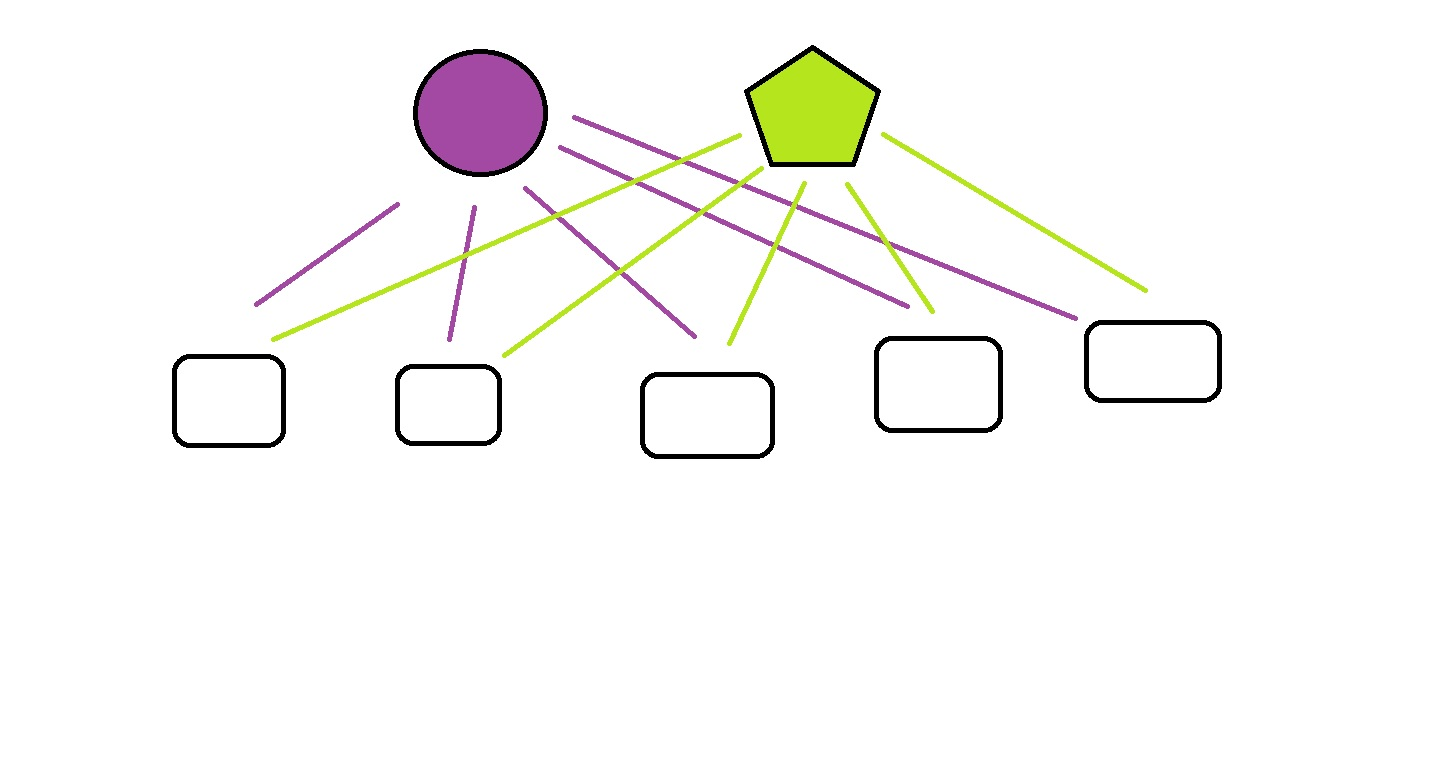
\includegraphics[width=16cm]{assets/NSD.jpg}\\
	\newpage
	  $\underline{\hspace{3cm}}$\\
	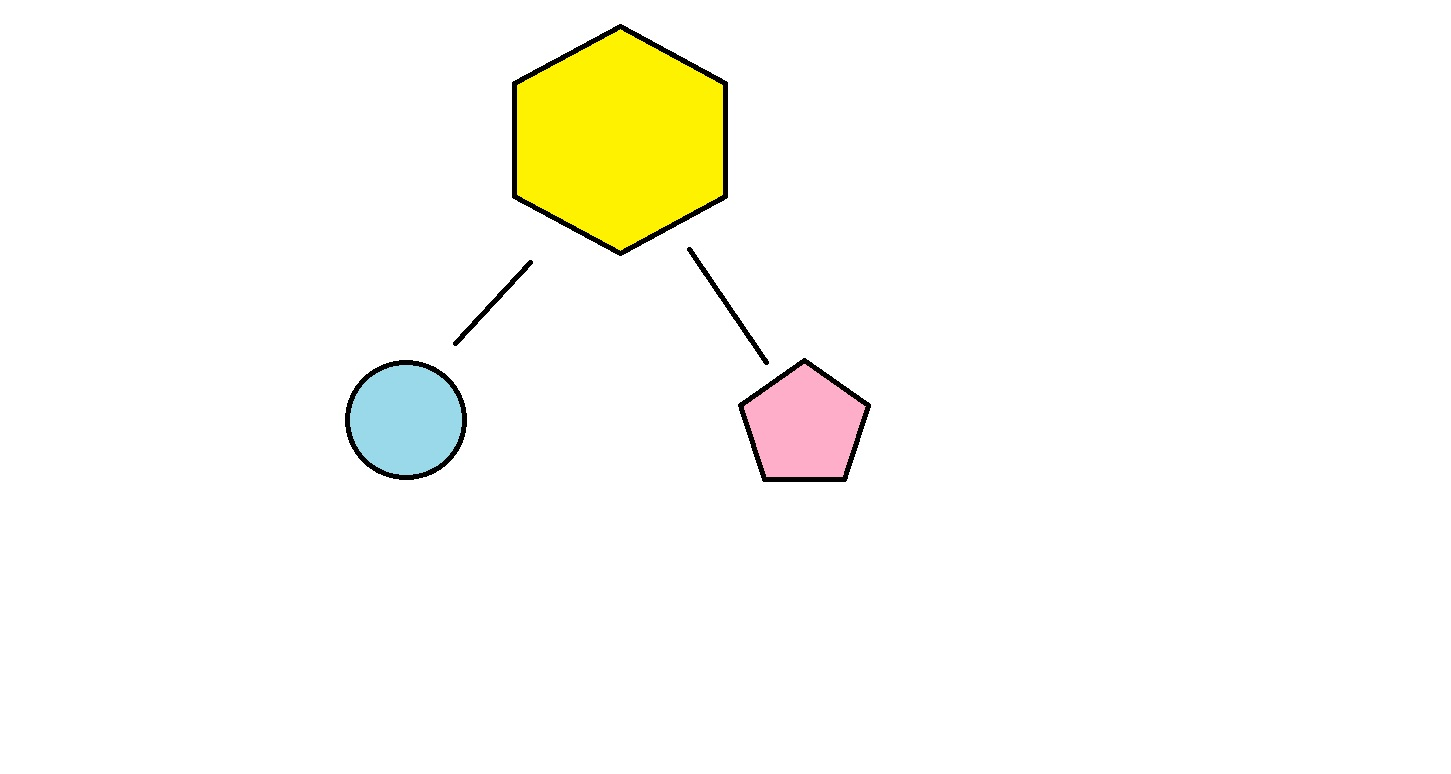
\includegraphics[width=16cm]{assets/nsn.jpg}\\
	
	Teraz si ukážeme nejaké vzorové príklady.
	
	\textbf{Príklad 1.} Babička má 8 lízaniek a 28 cukríkov a chce vedieť, do najviac koľkých balíčkov ich vie rozdeliť. Poraďme babičke! :{)}\\
	
	\textbf{Riešenie:} Keďže chceme rozdelovať veci do skupín, hľadáme NSD(8, 28). To číslo už dopočítaj a dopíš sem: $\underline{\hspace{1cm}}$. \\
	
	\textbf{Príklad 2.} Máme 2 lode, obe vyrážajú z prístavu o 11:00. Loď A vyráža každých 15 minút a loď B každých 25 minút. Zisti, kedy sa prvýkrát stretnú.\\
	
	\textbf{Riešenie:} V časovom úseku, kedy sa stretnú, každá z nich už niekoľkokrát vyrazila. Z toho vyplýva, že dĺžku tohoto úseku vieme vydeliť 15-timi aj 25-timi. Takže nás zaujíma nsn(15, 25), ten túto podmienku spĺňa. Výsledkom je potom číslo $\underline{\hspace{2cm}}$.\\
	
	\textbf{Príklad 3.} Anička má 20 jabĺk a 30 marhúľ a chce z nich urobiť koláče. Ale chce ich vyrobiť čo najviac. Koľko ich vie upiecť?\\
	
	\textbf{Riešenie:} Anička chce vlastne deliť ovocia na skupiny, takže chce vedieť NSD(20, 30), to bude počet koláčov, do koľých ich vie najviac rozdeliť. Výsledok je $\underline{\hspace{2cm}}$\\
	
	\textbf{Príklad 4.} Keď učiteľ telocviku nechá nastúpiť študentov do 6-radu a 8-radu, nikto nevystáva. Koľko študentov je v triede?\\
	
	\textbf{Riešenie:} Keďže ich vie rozdeliť do 6-radu aj 8-radu, tak tento počet musí byť deliteľný 6-mi aj 8-mi, preto hľadané číslo je nsn(6, 8). Výsledok je $\underline{\hspace{2cm}}$.\\
	
	\textbf{Príklad 5.} Ferko má 24 modrých pier, 16 zelených a 44 červených. Chce vedieť, na koľko skupín ich vie najviac rozdeliť. Koľko ich bude? Koľko pier daných farieb bude v skupinách?
	
	\textbf{Riešenie:} Opäť delíme veci do meších skupiniek, takže hľadáme NSD(24, 16, 44), čo je $\underline{\hspace{2cm}}$. Ak chceme vedieť, koľko bude v skupinách, vydelíme počty NSD-čkom. Modrých pier: $\underline{\hspace{2cm}}$, zelených: $\underline{\hspace{2cm}}$ a červených: $\underline{\hspace{2cm}}$.
	
	\textbf{Príklad 6.} 3 lode vyrážajú každých 12, 15 a 20 minút. Prvýkrát vyrážajú o 12:30. Kedy sa prvýkrát stretnú?
	
	\textbf{Riešenie:} Hľadáme časový úsek, kam sa zmestí 12, 15 aj 20 minút, takže hľadáme nsn(12, 15, 20). Výsledok je: $\underline{\hspace{2cm}}$. Teda prvýkrát sa stretnú $\underline{\hspace{2cm}}$.
	
	\textbf{Príklad 7.} Zoberme si lode z predchádzajúcej úlohy. Zaujíma nás, koľkokrát sa stretnú do 18:00.
	
	\textbf{Riešenie:} Zaujíma celočíselný podiel úseku od 12:30 do 18:00. Keď zistíme túto dĺžku v minútach, urobíme len celočíselný podiel tohto čísla a nsn z predchádzajúcej úlohy (urobíme delenie so zvyškom a výsledkom je len celá časť). Takže sa stretnú $\underline{\hspace{1cm}}$-krát. 
	
	
	
	\newpage
	\section{Racionálne čísla a zlomky}
	
	\subsection{Definícia}
	\qquad Do definície dopíš nasledovné slová: \textbf{celých čísel, nule, čitateľ, menovateľ, pomer, zlomok},a zisti, aké značenie sa používa pre racionálne čísla. \newline
	
	\textbf{Definícia:} Racionálne číslo je také číslo, ktoré vieme zapísať ako $\underline{\hspace{2cm}}$ 2 $\underline{\hspace{3cm}}$ $x$ a $y$, zápisujeme to ako $\frac{x}{y}$, tento tvar sa potom nazýva $\underline{\hspace{2cm}}$. Číslo $x$ sa nazýva $\underline{\hspace{2cm}}$ (lebo ho prečítame prvé) a $y$ sa nazýva $\underline{\hspace{2cm}}$ (lebo dáva zlomku meno) treba si dať ale potom pozor na to, že menovateľ nesmie byť rovný $\underline{\hspace{2cm}}$. Značenie pre racionálne čísla je $\underline{\hspace{1cm}}$.\\
	
	
	Z tabuľky doplň slová do textu na správne miesta.\\
	\begin{table}[!hbt]
		\centering
		\begin{tabular}{|ccc|}
			\hline
			základnom& súdeliteľné& nesúdeliteľné\\
			rozširovanie& krátenie& $\mathbb{Q}$\\
			\hline
		\end{tabular}
	\end{table}
	
	\begin{itemize}
		\item zlomok $\frac{x}{y}$, kde NSD(x, y) = 1, sa nazýva zlomok v $\underline{\hspace{2cm}}$ tvare.
		\item vynásobenie čitateľa aj menovateľa rovnakým \textbf{nenulovým} číslom sa nazýva $\underline{\hspace{2cm}}$. Uvedom si, že táto operácia nemení hodnotu zlomku.
		\item opačná operácie, teda vydelenie čiateľa aj menovateľa tým istým \textbf{nenulovým} číslom, sa nazýva $\underline{\hspace{3cm}}$.
	\end{itemize}
	
	
	%\subsection{Rozširovanie zlomkov}
	
	
	\subsection{Cvičenia}
	\qquad Vyššie bolo spomenuté krátenie a rozširovanie zlomkov, Okrem toho sme si definovali aj zlomok v základnom tvare. Ale čo, ak zlomok v základnom tvare nie je? Existuje na to veľmi jednoduchý postup:\\
	\begin{enumerate}
		\item Nájdi ľubovoľného spoločného deliteľa čitateľa a menovateľa.
		\item Vykráť zlomok týmto deliteľom.
		\item Ak je zlomok v základnom tvare, sme hotoví. Inak znovu aplikuj rovnaký postup.
	\end{enumerate}
	
	V nasledujúcej tabuľke máš dané zlomky a celé nenulové čísla, ktorými ich máš rozšíriť v zátvorkách. Do druhého stĺpca zapíš výsledky.
	\newline
	\begin{table}[!hbt]
		\centering
		\begin{tabular}{|l|l|}
			\hline
			$\frac{5}{3}$ (-3)&\hspace{2cm} \\
			\hline
			$\frac{-7}{2}$ (23)&\hspace{2cm} \\
			\hline
			$\frac{9}{-31}$ (11)&\hspace{2cm} \\
			\hline
			$\frac{-5}{-83}$ (-6)&\hspace{2cm} \\
			\hline
			$\frac{22}{21}$ (4)&\hspace{2cm} \\
			\hline
			$\frac{51}{13}$ (36)&\hspace{2cm} \\
			\hline
			$\frac{16}{93}$ (7)&\hspace{2cm} \\
			\hline
		\end{tabular}
	\end{table}
	\newline
	
	Teraz budeš mať v tabuľke zlomky a tvojou úlohou je ich previesť do základného tvaru, okrem NSD využi krátenie, ak bude čitateľ aj menovateľ záporný. Kladné čísla sú pri zlomkoch preferované.\\
	
	\newpage
	\subsection{Operácie so zlomkami}
	\begin{enumerate}
		\item \textbf{Sčitovanie/odčitovanie s rovnakými menovateľmi}: V tomto prípade ide o jednoduchý postup, keďže sa oba zlomky skladajú z rovnako veľkých častí. Máme teda 2 zlomky $\frac{x}{m}$ a $\frac{y}{m}$, ich súčet je potom súčet čitateľov $\frac{x+y}{m}$ (pri rozdieli tam je len rozdiel čitateľov).
		
		\item \textbf{Násobenie zlomkov:} $\frac{a}{b} \cdot \frac{x}{y} = $
		\item \textbf{Delenie zlomkov:} $\frac{a}{b} \div \frac{x}{y} = $
		\item \textbf{Sčitovanie a odčitovanie zlomkov s rôznymi menovateľmi:} Máme 2 zlomky  $\frac{a}{b}, \frac{x}{y}$ a chceme ich sčítať, keďže nemáme rovnaké menovatele, nemôžeme len tak sčítať čitatele. V tomto prípade sa postupuje rak, že to prevedieme na spoločný menovateľ, ktorým bude číslo $b \times y$. Dostaneme teda rovnosť $\frac{a}{b} + \frac{x}{y} = \frac{nieco}{b \cdot y}$. Chceme vedieť, čo je nič, aby sme pri daných 2 zlomkoch dosiahli menovateľ $b \cdot y$, prvý zlomok rozšírime číslom y a druhý číslom b. Následne teda dostaneme:
	\end{enumerate}
	\begin{center}
		\LARGE $\frac{a \cdot y}{b \cdot y} + \frac{x \cdot b}{y \cdot b} = \frac{a \cdot y + x \cdot b}{b \cdot y}$.
		
	\end{center}
	
\end{document}
